\chapter{Introduction}

	Ever since the Industrial Revolution, the energy consumption of the World has done nothing but rise over time. \cite{bibid} This rise in energy consumption correlates well with a rise in quality of life seen throughout the years. \cite{bibid} We will therefore take it as an axiom that the continued increase in energy consumption is not only inevitable but also desirable for the Net Good of Humanity. It is worth noting that the distribution of energy consumption and the efficiency of energy consumption are both extremely important topics in and of themselves, but unfortunately are beyond the scope of this discussion. This situation means that energy production must also continue to rise so as to meet the growing demand.
	
	Unfortunately, time has quickly shown that our current forms of energy production are not sustainable. \cite{bibid} The vast majority of energy produced today comes from \emph{fossil fuels}; materials such as coal, oil, and natural gas. \cite{bibid} These fuels are formed by natural processes that take place over time periods on the order of millions of years. \cite{bibid} Due to this extremely long production time, our consumption has far outpaced it leading to these fuels being classified as \emph{non-renewable}. \cite{bibid} This would not be intrinsically bad if the source was effectively infinite, but most research estimates that these resources can only last on the order of 100 years at current consumption rates. \cite{bibid} This finite supply has already lead to a handful of \emph{energy crises} over the years. \cite{bibid}
	
	Even more important than the limited theoretical supply is the environmental impacts of these fuels. Massive amounts of carbon dioxide (CO$_2$) are released into the environment every year due to the burning of fossil fuels. \cite{bibid} Research has repeatedly shown that this emission is having harmful, non-reversible impacts on the environment. \cite{bibid} Several countries have deemed this to be undesirable and have taken a variety of actions to reduce future releases of CO$_2$. \cite{bibid} These actions serve to limit the amount of fossil fuels that can be burnt, which even further limits the ability of fossil fuels to meet our growing demand. It is therefore, extremely desirable to develop alternative \emph{renewable} energy sources that can meet our demands without producing exorbitant amounts of CO$_2$.
	
	Thankfully, there are a handful of different energy sources that meet these requirements, each with their own advantages and disadvantages. They are hydroelectric, wind, solar, nuclear fission, and nuclear fusion. 
	
	\subsubsection{Hydroelectric Power}
	
		Hydroelectric power is generated from dams built along the path of rivers. Gravity forces the water to descend through the dam where it passes through and spins a turbine. The spinning turbine drives an electric generator creating the electricity.
		
		\begin{figure}[h!]
			\centering
			\includegraphics[scale=0.175]{ThreeGorgesDam}
			\caption[Three Gorges Dam]{The Three Gorges Dam in Sandouping, China is the world's largest power generating station of any kind. It generates 22,500 MW of electricity from the Yangtze River. \cite{Image_ThreeGorgesDam}}
		\end{figure}
	
		Hydroelectric is considered a renewable resource because the source for a given dam is effectively infinite. \cite{bibid} Because there is no steam involved, they are highly efficient, only having to convert kinetic energy to electricity. \cite{bibid} Dams generate larges amounts of power at competitive costs to fossil fuels \cite{bibid} and are generally always available. \cite{bibid} Additionally, they can be highly flexible with their power outputs allowing them to follow variable demands. \cite{bibid} All of this without the consequence of releasing CO$_2$ into the environment. \cite{bibid}
		
		The primary disadvantage of hydroelectric power is the number of suitable locations for dams is finite. \cite{bibid} While for most countries, there is still room for expansion today \cite{bibid}, it will not be sufficient to meet growing power demands indefinitely. So while hydroelectric is an extremely attractive source of clean renewable energy, it alone cannot serve to meet our energy needs.
		
	
	\subsubsection{Wind Power}
	
		Wind power is generated by large windmills whose blades turn when struck by wind. The spinning blades ultimately turn a turbine which goes on to produce electricity  through an electric motor. \cite{bibid}
		
		\begin{figure}[h!]
			\centering
			\includegraphics[scale=0.25]{windmillFarm}
			\caption[San Gorgonio Pass Wind Farm]{San Gorgonio Pass Wind Farm located in Riverside County California. The farm consists of 3,218 units delivering a total of 615 MW. \cite{bibid} }
		\end{figure}
	
		Like hydroelectric, wind is clearly a renewable resource and windmills have no associated CO$_2$ production with operation. \cite{bibid} Like hydroelectric, no steam is involved in the energy conversion process so it can be made high efficient. \cite{bibid}
		
		Wind power does have a handful of disadvantages when compared to fossil fuels. First off, wind is not always available and when it is speeds are variable. This means wind cannot be used as a so called \emph{base load} energy source.\cite{bibid} Base load sources are those that can produce electricity nearly indefinitely to meet the minimum demand of the grid at all times. \cite{bibid} Wind's variable often unpredictable nature means the produced energy often needs to be stored in some way, increasing operational costs. \cite{bibid} Cost comparisons with fossil fuels vary, but generally wind is considered to be more expensive; although not intolerably so. \cite{bibid}
		
		Another disadvantage of wind power is it's energy density, the amount of energy it can produce per unit area required to operate. On average, a single windmill produces on the order of \todo{2 MW} while occupying an area on the order of \todo{1.5 acres} with a capability factor (fraction of time producing power) of roughly \todo{33\%}. \cite{bibid} For reference the average power consumption of the United States was \todo{482 GW} in 2018 \cite{bibid} meaning over \todo{$1500$} square miles (more than a Rhode Island of area) would be required to power the country on wind alone. \todo{Sources vary greatly on this, consider removing.}
		
		One final disadvantage of wind power is the environmental impact it has. Windmills have been shown to be harmful to birds \cite{bibid} and are generally unattractive to humans aesthetically. \cite{bibid} Given the large volume they consume, this can quickly become problematic. 
		
		All in all, wind is a renewable energy source but has several issues with it's implementation. While it certainly can hold a place in the energy profile of a pure renewable energy grid, it cannot meet the demand reliably alone.
		
	
	\subsubsection{Solar Power}
	
		Solar power largely refers to a variety of technologies that convert radiation from the sun into electricity. \cite{bibid} While the exact method for extracting electricity varies between different technologies, for the purposes of this discussion they largely have the same advantages and disadvantageous.
		
		 \begin{figure}[h!]
		 	\centering
		 	%\includegraphics[keyvals]{imagefile}
		 	\caption{\todo{Solar Farm}}
		 \end{figure}
	 
	 	Like all the other forms of power generation mentioned thus far, the sun is clearly a renewable source of energy. And like the other renewable sources of energy, no CO$_2$ emissions are required in the conversion to electricity. 
	 	
	 	The disadvantages of solar power are very similar to those discussed with wind power. Solar power only works when the sun is out and even then, can be intermittently interrupted by inopportune weather. \cite{bibid} This makes solar power unattractive as a base load option and necessitates energy storage capabilities. 
	 	
	 	Like wind energy, solar also has a limited energy density. The sun's intensity on earth is about \todo{1.36 kW per square meter} and the efficiency of solar panels is of the order of \todo{15\%}. \cite{bibid} This means you'd need over \todo{1000 square miles} of constant sunlight to power the United States. Accounting for the capability factor brings this estimate up by a factor of 2 or 3. 
	
		Like wind, solar energy certainly has a place but cannot meet the growing energy demand on it's own.
	
	\subsubsection{Nuclear Fission}
	
		Nuclear fission refers to the process of fragmenting large atoms (typically masses of the order 200 amu) into smaller constituents. \cite{bibid} This releases a significant amount of energy (the physics of which we'll discuss in Section \ref{sec:Physics of Nuclear Energy}) which can then be used to heat water and generate electricity through the well known Carnot cycle. \cite{bibid} In fact, the way electricity is produced from nuclear fission is exactly identical to typical fossil fuel plants, the only difference being the source of heat.
		
		\begin{figure}[h!]
			\centering
			%\includegraphics[keyvals]{imagefile}
			\caption{\todo{Nuclear Power Plant}}
		\end{figure}
		
		When compared to fossil fuels, nuclear fission power has a couple of key advantageous. Firstly, fission generates no CO$_2$ making it a source of clean energy. \cite{bibid} Secondly, the energy density of nuclear fission is orders of magnitude above that of fossil fuels. The potential energy density of UO$_2$ (the fuel used in nuclear reactors) is roughly $7.1\times10^7$ MJ/kg \cite{bibid}. The energy density for coal and methane is only 15 and 55 MJ/kg respectively. \cite{bibid} This means the costs of fuel is practically non-existent for nuclear reactors, with most of the costs being capital cost in constructing the reactor. \cite{bibid} Additionally, the costs of nuclear energy tends to be competitive with fossil fuels when balanced over the life of the reactor. \cite{bibid}
		
		Nuclear fission power also has a couple of advantageous over the traditional renewable energy sources as well. Unlike solar and wind, nuclear power excels as a base load energy production option, often running continuously for 18 months at a time. \cite{bibid} Nuclear power is also traditionally cheaper than solar and wind \cite{bibid}, although over recent years the two have become much more competitive. \cite{bibid} Unlike hydroelectric, expanding nuclear power is only limited by the high investment costs needed to build new plants. 
		
		There are, however, disadvantages associated with nuclear fission power. One is the public perception of it's safety is not remarkable after the accidents at Chernobyl, \cite{bibid} Three Mile Island, \cite{bibid} and Fukushima \cite{bibid}. While there are those that would debate that these examples are unfair representations \cite{bibid}, it is nevertheless true that public opinion continues to be a challenge for nuclear fission. Another disadvantage of this technology is the spent fuel is a extreme radiation hazard have half lives on the order of millions of years. \cite{bibid} While this spent fuel, as of yet, doesn't impact the environment, there is currently no long term plan in the United States on how to handle it. \cite{bibid} 
		
		As noted before, the capital costs of nuclear fission power are much greater than any other energy source. \cite{bibid} Additionally, the act of getting a reactor approved and built is rather lengthy, full of complications, and prone to delays. \cite{bibid} This significantly limits the number of potential investors who can or even who are willing to explore nuclear power. This makes expansion fundamentally difficult. 
		
		Another disadvantage is nuclear fission is (by many accounts) not a true renewable energy source. \cite{bibid} The current most common and cheapest fuel cycles are extremely wasteful. The uranium must be enriched, so only about 10\% of uranium mined out of the ground makes it into the reactor. Of this, roughly 5\% is actually utilized for fission before becoming spent fuel. \cite{https://www.world-nuclear.org/information-library/nuclear-fuel-cycle/introduction/nuclear-fuel-cycle-overview.aspx} Uranium resources used this way at current consumption rates can last on the order of hundreds of years. \cite{bibid} In reality, there are other more efficient fuel cycles that can extend our resources to several thousand years but these come with costs and risks that are beyond the scope of this discussion. \cite{bibid}
		
		One final disadvantage is the concept of nuclear proliferation which, in this context, refers to the idea of a rogue and/or unstable organization acquiring nuclear weapon material somewhere in the fuel cycle. \cite{bibid} In the wasteful cycle we mentioned before, this risk is fairly minimal. However, any efforts to reprocess spent fuel to more efficiently utilize it inherently involves the separation and concentration of plutonium. \cite{bibid} Extreme care must be taken to ensure that none of this plutonium is diverted from the fuel cycle which presents a very real and challenging risk.
		
		In conclusion, nuclear fission power holds extreme promise as an expandable base load power source that does not emit CO$_2$. It does, however, come with a vast amount of non trivial challenges. It certainly will play an important role in any carbon free energy profile, so long as the challenges can be appropriately addressed.
		
		
	\subsubsection{Nuclear Fusion}
	
		Nuclear fusion is very similar to nuclear fission except it involves combining light atoms (masses of order 1 amu) together. \cite{bibid} Like with fission, this generates enormous amounts of energy which could be used as a heat source in any variety of thermodynamic cycles. Unlike with the other technologies discussed thus far, nuclear fusion power has yet to be scientifically demonstrated. \cite{bibid}
		
		\begin{figure}[h!]
			\centering
			%\includegraphics[keyvals]{imagefile}
			\caption{\todo{Nuclear Fusion Experiment}}
		\end{figure}
		
		Nuclear fusion shares many of the advantages of nuclear fission. Like fission, nuclear fusion power would emit no CO$_2$ into the environment and it has an extremely high fuel energy density. If one were to consider the fusion of hydrogen isotopes tritium (T) and deuterium (D), the energy density is of order 3.5 MeV per amu compared to fission of $^{235}$U which is more like 0.85 MeV per amu. \cite{bibid} It's also possible to simply fuse D with D which is found in trace amounts in water (H$_2$O). With this in mind, a perhaps more fair comparison is the potential fusion energy density of H$_2$O which is roughly $3\times10^3$ MJ/kg; still orders of magnitude above coal and methane. \cite{bibid}
		
		Like hinted at, the primary source of fuel for any nuclear fusion power scheme would be hydrogen. There are other reactions that would involve other fuels such as helium or even boron, but we shall ignore those for now. \cite{bibid} Deuterium is naturally present in water of which there is a significant abundance on Earth. \cite{bibid} Any fusion power plant that used deuterium alone would certainly be considered effectively renewable due to the massive water reserves available in oceans. In reality, the first generation of nuclear fusion reactors would rely on tritium which does not exist naturally on Earth. It can, however, be produced from $^6$Li or even deuterium via neutron bombardment. \cite{bibid} Thankfully, lithium is also plentiful on Earth, not so much as to be considered renewable, but enough that it could last tens of thousands of years at current electrical consumption rates. \cite{bibid} 
		
		A unique advantage of nuclear fusion is it's intrinsic safety. The reason fusion power has yet to be scientifically demonstrated is exactly the same thing that makes it so safe. Nuclear fusion requires the containment of fuel hotter than the center of the Sun, which is an extreme scientific and engineering challenge. \cite{bibid} While this may sound unsafe, it means that the these extreme temperatures must be maintained for the fusion reaction to continue. Any failure mode that would result in a compromised containment which would immediate halt any additional fusion reactions. In addition, by design, fusion reactors only have very small amounts of fuel in the "core" at any given time. This is distinctly different from fission where a reactor is loaded with enough fuel such that 5\% of it will last 18 months. \cite{bibid}.  What this means is that even if all of the fusion fuel were to be consumed in a runaway reaction, the total energy released would be minimal. In Inertial Confinement Fusion (ICF) schemes, all of the fuel in current designs translates to roughly 100 sticks of dynamite which is certainly containable with modern containment structures. \cite{bibid}
		
		Another advantage that nuclear fusion would have over nuclear fission, is the lack of long lived radioactive spent fuel. For fusion, the spent fuel is generally some combination of hydrogen and helium both of which are completely inert to the environment. \cite{bibid} In the case of DD fusion, the spent fuel would actually be radioactive (in the form of tritium), but the half-life is on the order of 10 years, not millions. \cite{bibid} Nuclear fusion does emit high energy neutrons that would go on to activate structural materials. These activated structural materials would half half-lives on the order of hundreds of years, again much lower than that of spent fuel from nuclear fission. \cite{bibid}
		
		The primary disadvantage of nuclear fusion is quite clear; the technology does not exist. Unlike with nuclear fission power, nuclear fusion power has been out of reach for nearly 70 years. \cite{bibid} This is because the technical demands associated with trying to contain a plasma hotter than the Sun here on Earth is quite challenging. To date, the technical viability of fusion has never been demonstrated outside of nuclear weapons and, infact, many attempts have failed. \cite{bibid} All of that said, the performance of nuclear fusion experiments has shown a steady increase over time suggesting that success will come inevitably. \cite{bibid}
		
		Another very real disadvantage of nuclear fusion is the expected costs. Nuclear fusion facilities are currently very expensive to operate and would never be able to generate electricity competitively. \cite{bibid} For example, the National Ignition Facility (NIF) spends roughly \todo{one million USD} per experiment. \cite{bibid} The maximum theoretical yield from one of these experiments would generate less than 6 USD worth of electricity at current costs. \cite{bibid} Using instead the maximum credible yield combined with the fact that energy will be loss converting to electricity brings this estimate below 1 USD. \cite{bibid} While technology will expected to lower costs over time and electricity prices are likely to rise, the fact remains that the current gap is many orders of magnitude away.
		
		In summary nuclear fusion power holds great potential as a future base load power source with seemingly no safety risk or negative consequences. It's potential is locked entirely by technical and scientific issues that require more study and research. While nuclear fission is certainly sufficient to supply to World's clean energy needs in years to come, the vast potential of nuclear fusion justifies it's continued investigation. We will therefore spend the introduction of this thesis discussing the basic theory and the current state of nuclear fusion efforts. 
	
	\section{Physics of Nuclear Energy}
\label{sec:Physics of Nuclear Energy}

	The energy released from any reaction is dictated by Einstein's famous equation: \cite{bibid}
	%
	\begin{equation}
		E = mc^2
	\end{equation}
	%
	where $E$ is the so called rest mass energy of an object with mass $m$ and $c$ is the speed of light. To calculate the energy release of a reaction, one simply subtracts the rest mass energy of the initial state from the final state such that:
	%
	\begin{equation}
		\Delta E \equiv Q = \left(\sum m_i - \sum m_f \right) c^2
		\label{eq:reactionEnergyRelease}
	\end{equation}
	%
	Here $m_i$ is the masses of any initial components (particles in our context) and $m_f$ is the masses of any final components. It is a common misconception that equation \ref{eq:reactionEnergyRelease} only applies to nuclear reactions, but in reality chemical reactions are described by the same physics. Some example reactions are shown in Table \ref{tab:reactionEnergyReleases}. 
	
	\begin{table}[!h]		
		\caption{Mass differences and energy released by various reactions}
		\centering
		\tabulinesep = 1.5mm		
		\begin{tabu}{|c|c|c|c|}
			\hline
			Reaction & Type & $\left(\sum m_i - \sum m_f \right)$ & $Q$ \\
			\hline
			p + e$^-$ $\rightarrow$ $^1$H & Recombination & $1.46\times10^{-8}$ amu & 13.6 eV\\
			n + $^{235}$U $\rightarrow$ $^{140}$Xe + $^{94}$Sr + 2n & Fission & 0.198 amu & 184.7 MeV\\
			$^{2}$H + $^{3}$H $\rightarrow$ $^{4}$He + n & Fusion & 0.0189 amu & 17.6 MeV \\ 
			\hline
		\end{tabu}
		\label{tab:reactionEnergyReleases}
	\end{table}

	For us to produce energy, we ultimately seek to find reactions that produce large $Q$. To do this we need reactants with large $m_i$ relative to the $m_f$ of the products. To aid in determining this, the masses of several isotopes are shown plotted in Figure \ref{fig:massPerNuclide}.
	
	
	\begin{figure}
		\centering
		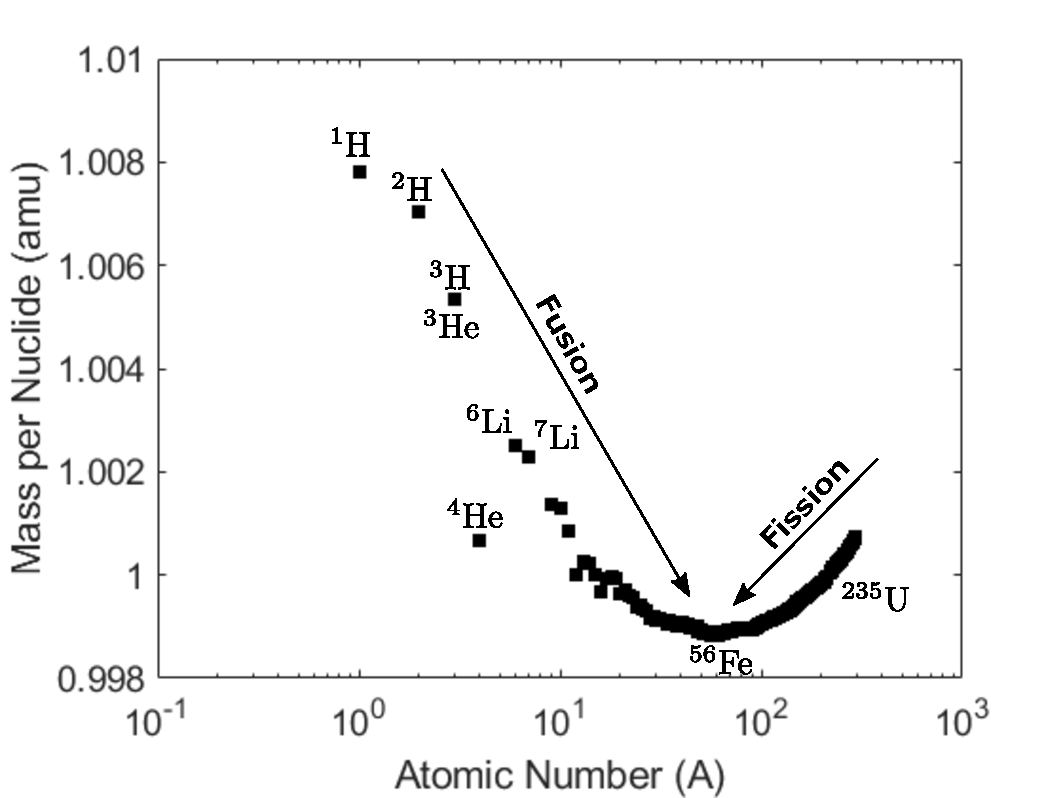
\includegraphics[scale=0.7]{massPerNuclide}
		\caption{Mass per nuclide of various isotopes. All exothermic fusion reactions must occur between isotopes lighter than $^{56}$Fe and all exothermic fission reactions must occur between isotopes heavier than $^{56}$Fe. }
		\label{fig:massPerNuclide}
	\end{figure}

	As we can see, the isotope with the smallest mass per nuclide is $^{56}$Fe. It is considered the most efficiently bound nuclide since it's corresponding rest mass energy per nuclide is lower than any other isotope. This means that for any isotopes lighter than ${^{56}}$Fe, we can gain energy by combining them (fusion) into heavier isotopes. Similarly, we gain energy by breaking up isotopes (fission) with mass greater than $^{56}$Fe. It is interesting to note the local minimum mass per nuclide of $^4$He. Due to it's unique position, fusion reactions that produce it will be particularly energetic. Interestingly, it also means that the fission of $^6$Li is uniquely exothermic. The exact reason for why isotope masses behave in this way is a topic of nuclear physics beyond the scope of this discussion. 
	
	Moving forward, we will adopt short-hand notations for a few light isotopes of particular interest to fusion. These isotopes are listed in Table \ref{tab:isotopeShorthands}.
	
	\begin{table}[h!]
		\centering
		\tabulinesep = 1.5mm
		\caption{Short hand notations for a few light isotopes of particular interest to nuclear fusion}
		\begin{tabu}{|c|c|c|}
			\hline
			Name & Proper Notation & Short Hand \\\hline
			Deuteron & $^2$H & D \\
			Triton & $^3$T & T \\
			Alpha Particle & $^4$He & $\alpha$ \\
			\hline 
		\end{tabu}
		\label{tab:isotopeShorthands}
	\end{table}
	
	With this notation in mind, there are a few fusion reactions that are of particular interest for energy production. 
	
	\begin{eqnarray}
			\text{D + D} &\rightarrow& \text{T + p + 4.03 MeV}  \label{eq:DDp}\\
			\text{D + D} &\rightarrow& ^3\text{He + n + 3.27 MeV} \label{eq:DDn}\\
			\text{D + T} &\rightarrow& \alpha \text{ + n + 17.6 MeV} \label{eq:DTn}\\
			\text{D + } ^3\text{He} &\rightarrow& \alpha \text{ + p + 18.3 MeV} \label{eq:D3Hep} \\
			\text{p + } ^{11}\text{B} &\rightarrow& 3\alpha	\text{ + 8.7 MeV} \label{eq:p11B}		
	\end{eqnarray}

	These reactions are primarily chosen due to the availability of the reactants, the amount of energy released, and the ease to which they can be made to fuse. The last of these criteria is described by the reaction's fusion cross-section ($\sigma$). Cross sections are essentially the probability (normalized for density and path length) that two particles will interact, or in our case fuse. As such, the cross section determines the reaction rate between two species. Formally the volumetric reaction rate between species 1 and 2 is given by:  
	%
	\begin{equation}
		\mathcal{R}_{12} = \int dv_1^3 \int dv_2^3 f_1(\vec{v}_1) f_2(\vec{v}_2) \sigma_{12} \left|\vec{v}_1 - \vec{v}_2\right|
		\label{eq:reactionRate}
	\end{equation}
	%
	where $f_1$ and $f_2$ are the velocity distribution functions of species 1 and 2 respectively and $\vec{v}_1$ and $\vec{v}_2$ are the velocities of species 1 and 2 respectively. The cross sections for all of the listed reactions are shown in Figure \ref{fig:crossSections}. 
	
	\begin{figure}[h!]
		\centering
		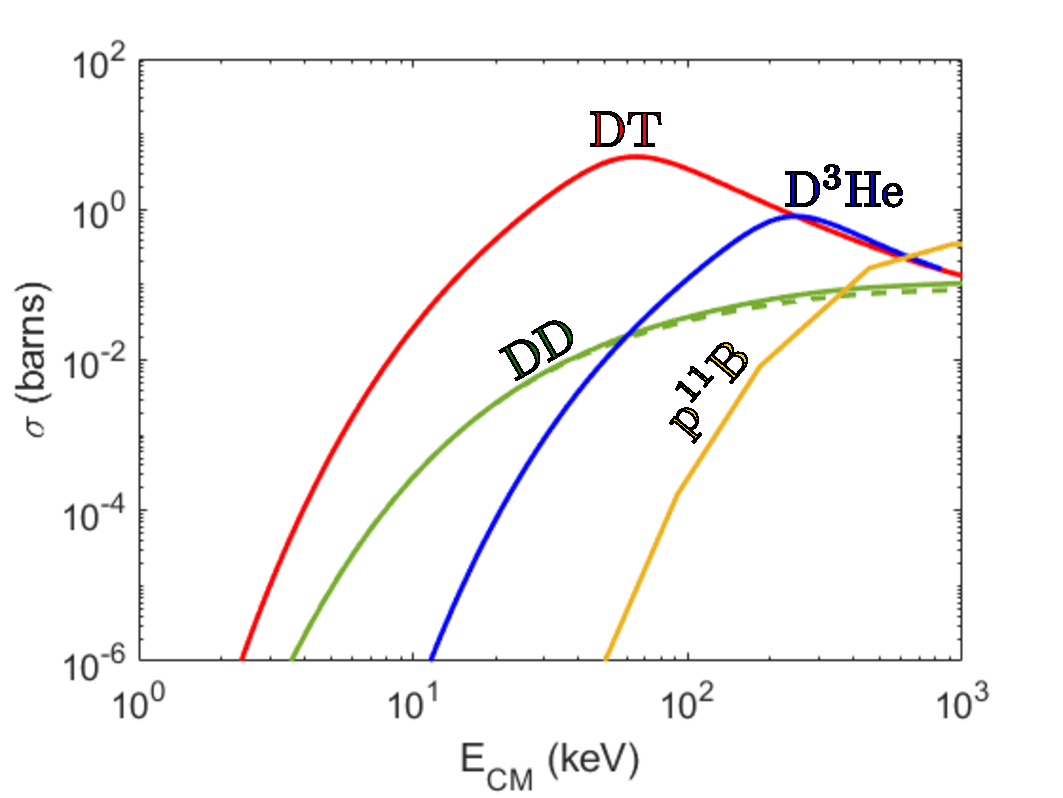
\includegraphics[scale=0.7]{crossSections}
		\caption[Fusion Cross-Sections]{Cross sections of various fusion reactions consider for fusion energy. The cross sections for equations \ref{eq:DDp} - \ref{eq:p11B} are shown as green, green, red, blue, and yellow curves respectively. The cross sections for equations \ref{eq:DDp} and \ref{eq:DDn} are nearly identical up until very high energies. Equation \ref{eq:DDp} is dashed and equation \ref{eq:DDn} is solid. Cross sections here are plotted as a function of their center of mass energies. }
		\label{fig:crossSections}
	\end{figure}

	As we can see there are many orders of magnitude separating the cross-sections of these reactions depending on the center of mass energy. DT fusion (equation \ref{eq:DTn}), is by far the easiest to achieve having a max cross section of about 5 barns. For context this is roughly 100 times less than the thermal fission cross section of $^{235}$U. Following DT, DD fusion (equations \ref{eq:DDp} and \ref{eq:DDn}) is the next easiest to achieve at reasonable energies. For this reason, most major fusion experiments in the world aim for DT fusion as this will be the reaction that powers the first generation of nuclear fusion reactors. The other reactions listed have their advantages such as higher fuel availability or being aneutronic (emitting no neutrons) but will be reserved for second or third generation fusion reactors.
	
	An important thing to note about these cross sections is the rather high center of mass energies required to achieve them. For reference, the fission cross section quoted previously occurs at room temperature energies (0.0253 eV) whereas the maximum DT cross section occurs at about 65 keV. This corresponds to temperatures of 750 million degrees Celsius (1.3 billion degrees Fahrenheit). This is because all fusion reactions require combining nuclides that are both positively charged leading to a Coulomb repulsion that can only be overcome with extreme energies. This Coulomb repulsion is also why the fusion of hydrogen atoms (who have the lowest possible charge) requires less energy than the reactions involving helium or boron. This is the primary challenge of nuclear fusion; creating and maintaining these extreme conditions. 
	
	Perhaps the most naive way to achieve nuclear fusion is through the acceleration of particles into a solid target. In fact this works remarkably well and is still the source of many fusion experiments to date. However, this approach to fusion is inefficient and cannot be used to generate net power. This is because the accelerated particle loses energy to Coulomb collisions with the solid target at a rate much higher than the fusion rate. A 100 keV triton, for example, travels less than 1 um into a solid target of pure deuterium before loosing all of its energy. This is compared to the 6000 um "mean fusion path length" one calculates from a 5 barn cross section. This means the fusion efficiency no better than 1/6000 (in fact it is much lower) but our energy gain per reaction is only 17.6 MeV / 100 keV = 176. 
	
	This necessitates thermonuclear fusion approaches, an approach in which the entire system is sufficiently heated to fusion viable temperatures. In a thermal system, internal Coulomb collisions are no longer a loss as they simply maintain the temperature. This is why most major approaches to fusion energy gain are thermonuclear. There are a few notable exceptions to this, but they're beyond the scope of this discussion. 
	
	The next question to address is, how hot does a thermonuclear system need to be in order to generate fusion power? To answer this we must return to equation \ref{eq:reactionRate} and replace $f_1$ and $f_2$ with thermal Maxwellian distributions. 
	%
	\begin{equation}
		\begin{split}
			\mathcal{R}_{12}  & = \frac{n_1n_2}{1+\delta_{12}} \left(\frac{m_1 m_2}{4\pi^2T_1T_2}\right)^{3/2} \int dv_1^3 \int dv_2^3  e^{-\frac{m_1|\vec{v}_1|^2}{2T_1}} e^{-\frac{m_2|\vec{v}_2|^2}{2T_2}} \sigma_{12} \left|\vec{v}_1 - \vec{v}_2\right| \\
			& = \frac{n_1n_2}{1+\delta_{12}} \left<\sigma v\right>_{12}
		\end{split}
		\label{eq:reactionRateThermal}
	\end{equation}
	%
	Here $n_1$ and $n_2$ are the number densities of species 1 and 2, $\delta_{12}$ is a Dirac delta to avoid double counting if species 1 and 2 are the same, $m_1$ and $m_2$ are the masses of species 1 and 2, and $T_1$ and $T_2$ are the temperatures (in units of energy) of species 1 and 2. Note that in the second line we have defined away the integrals into the term $\left<\sigma v\right>_{12}$ which is called the \emph{reactivity}. Note that this is very different than the concept of reactivity from nuclear fission. In nuclear fusion, reactivity is the density normalized reaction rate of species 1 and 2 at a given temperature. Reactivities for all of the discussed reactions is shown in Figure \ref{fig:reactivities}.  
	
	\begin{figure}[h!]
		\centering
		\includegraphics[scale=0.7]{reactivities}
		\caption[Fusion Reactivities]{Reactivities of various fusion reactions considered for fusion energy. The reactivities for equations \ref{eq:DDp} - \ref{eq:p11B} are shown as green, green, red, blue, and yellow curves respectively. The reactivities for equations \ref{eq:DDp} and \ref{eq:DDn} are nearly identical up until very high temperatures. Equation \ref{eq:DDp} is dashed and equation \ref{eq:DDn} is solid.  }
		\label{fig:reactivities}
	\end{figure}
	
	
	\section{Inertial Confinement Fusion}
\label{sec:ICF}

	Traditionally, fusion power approaches aim to create plasma conditions hot enough to allow nuclear fusion and then maintain these conditions long enough (ideally indefinitely) to get a sufficient amount of power out. In these schemes, additional fuel is added to the system as fuel burns away without ever transitioning away from the desired plasma conditions. 
	
	Another approach is a pulsed scheme, one where a single component of fuel is brought to the desired temperature and density until all or most of it burns away. Instead of maintaining extreme plasma conditions, they would be recreated each time for each individual component of fuel. This process would be repeated at some frequency in order to achieve some desired power output.
	
	One immediate problem with this approach is the limited energy gain available. As we've seen from Figure \ref{fig:reactivities}, nuclear fusion requires temperatures of order 10 to 20 keV and the total energy received (for DT) is 17.6 MeV. Assume we expend some energy to create a DT plasma with $n_D=n_T=n/2$ and we burn some fraction $f$ of the fuel. The fractional energy gain $G$ would be:
	%
	\begin{equation}
		G = \frac{E_{gain}}{E_{spent}} = \frac{fnQ}{3/2\left(n_DT + n_TT\right)} = \frac{Qf}{3T}
	\end{equation}
	%
	In the absolute best case scenario $f=100\%$ and taking $T=20$ keV, we achieve a gain of roughly 600. This may seem like a lot, but it's extremely limiting from an engineering standpoint as it represents the absolute best we can possibly do. Once you start to consider any realistic inefficiencies (40\% from Carnot, 10\% from the heating process, 50\% fuel utilization, etc) the potential energy profit starts to diminish rapidly. This approach of heating the entire fuel volume is often referred to as \emph{volume ignition}.
	
	To get around this, we consider a hybrid approach that we'll refer to as \emph{hot-spot ignition} in the center. In this pulsed power approach, we will still only interact with a single fuel component at a time but we'll only heat some fraction of it to fusion conditions. The remaining \emph{cold fuel} will be heated from the fusion power itself; specifically from the charged particle products. For DT fusion, this means that the $\alpha$ particles (which only carry 20\% of the energy) will heat the remaining cold fuel. This creates a runaway process in the form of a propagating burn wave throughout the entire fuel volume. See Figure \ref{fig:hotspot} for a diagram of this idea.
	
	\begin{figure}[h!]
		\centering
		\caption{\todo{Hot spot}}
		\label{fig:hotspot}
	\end{figure}

	We only need the hot-spot to generate enough energy to heat up the cold fuel immediately around it. A detailed calculate of this is not entirely straightforward but let's say a factor of 2 more energy than what is required to heat it. Accounting for the fact that $\alpha$s only carry 20\% of the energy means we need a hot-spot $G$ of about 10. This means we need to burn about $f_{HS}=3\%$. 
	
	Let's consider now, how long it will take to burn away this fraction of fuel. Taking equation \ref{eq:reactionRateThermal} we can write down the differential equation that governs rate of fuel burn:
	%
	\begin{equation}
		\dfrac{dn}{dt} = - \frac{n^2}{2}\left<\sigma v\right>_{DT}
	\end{equation}
	%
	Or in terms of $f$:
	%
	\begin{equation}
		\frac{df}{dt} = (1-f)^2\frac{n_0}{2}\left<\sigma v\right>_{DT}
	\end{equation}
	%
	where $n_0$ is the initial fill density of the fuel. If we assume $\left<\sigma v\right>$ is roughly constant over the burn, we can solve for $f$ to get:
	%
	\begin{equation}
		f = \frac{n_0\left<\sigma v\right>_{DT}\tau}{2 + n_0\left<\sigma v\right>_{DT} \tau}
		\label{eq:fuelFraction}
	\end{equation}
	%
	Where $\tau$ is the duration over which the fuel is able to burn. 
	
	As a side note, this equation is important because it highlights the three key components involved in burning fusion fuel; density ($n_0$), temperature ($\left<\sigma v\right>$), and confinement time $(\tau)$. It is similar to (but not the same as) the Lawson criteria in this way. All approaches to fusion must raise some combination of these three factors high enough in order to efficiently produce fusion power. Often the difference between approaches come down to what factor is being focused.

	For inertial confinement fusion (ICF), we seek to minimize the complications associated with confining these extreme condition plasmas. We do this by recognizing that any plasma will take a finite amount of time to disassemble itself. If we can get the plasma to a final state that burns sufficiently fast, that finite amount of time will be sufficient. We have yet to discuss how we'll get the plasma to this state, but let's explore the requirements associated with trying to do that.
	
	Without any confinement, a plasma will disassemble at a rate proportional to the acoustic ion sound speed:
	%
	\begin{equation}
		c_s = \sqrt{\frac{4T}{m_{DT}}}
	\end{equation}
	%
	Here we have assumed the electrons have the same temperature ($T_e$) as the ions. The fuel will continue burning so long as the density of the fuel has not sufficiently changed. Let's assume our fuel is all contained is a sphere of radius $R$ such that we can allow it to disassemble for some $\tau< R/c_s$ before the burn is too negatively effected. The exact value for $\tau$ is a bit arbitrary, and deserves detailed calculations, but most literature takes it to be $R/4c_s$. We can plug this into equation \ref{eq:fuelFraction} to show:
	%
	\begin{equation}
		\begin{split}
			f &= \frac{n_0\left<\sigma v\right>_{DT} R / 4c_s}{2 + n_0\left<\sigma v\right>_{DT} R / 4c_s} \\
			& = \frac{n_0m_{DT}R}{n_0m_{DT}R + \frac{8 c_s m_{DT}}{\left<\sigma v\right>_{DT}}}\\
			&= \frac{\rho R}{\rho R + H_B}
		\end{split}
		\label{eq:burnFraction}
	\end{equation}
	%
	Here we've defined a few new terms. $\rho R$ is the areal density of the plasma and $H_B$ is the so called \emph{burn parameter} which depends entirely on $T$. By defining our $\tau$ though the ICF approach, we have reduced our parameter space from three to two parameters. This means we can easily plot the fusion requirements for ICF schemes. 
	
		\begin{figure}[h!]
		\centering
		\includegraphics[scale=0.7]{fusionRequirements}
		\caption[ICF Fusion Requirements]{Areal density and temperature requirements to burn certain fuel fractions in ICF schemes. Dashed curves correspond to the hot-spot requirement of $f_{HS}=3\%$ and solid curves correspond to a cold-fuel high gain requirement of $f=30\%$. Different fuels are plotted as different colors. DT, D3He, DD, and p11B are plotted as red, blue, green, and yellow respectively.  }
		\label{fig:fusionRequirements}
	\end{figure}

	Using Figure \ref{fig:fusionRequirements} we can set some requirements for an ICF approach to achieve high gain. First we have the hot-spot ignition requirement from before of $f_{HS}=3\%$ which corresponds to an areal density of roughly 0.3 g/cm$^2$ at temperatures around 20 keV. For the rest of the fuel assembly, we want burn fractions high enough to produce substantial gain, but low enough to minimize the areal density requirement. For now let's take $f=30\%$ which corresponds to areal densities around 4-5 g/cm$^2$ for DT fuels. 
	
	The next question to address is how to get these areal densities. The most naive way would be to construct a fuel assembly with $R$ sufficiently large so as to meet the requirement. If we take the density of DT ice to be roughly 0.225 g/cm$^3$ we can achieve a $\rho R$ of 4.5 g/cm$^2$ with an $R=20$ cm. We can calculate the total energy released from this assembly:
	%
	\begin{equation}
		\begin{split}
			E_{tot} & \sim \mathcal{R}_{12} \times \tau \times V \times f \times Q \\
			& \sim \left(n_Dn_T\left<\sigma v\right>_{DT}\right) \times \left( \frac{R}{4 c_s}\right) \times \left(\frac{4}{3} \pi R^3\right) \times \left(\frac{\rho R}{\rho R + H_B}\right) \times Q \\
			& \sim \frac{\pi \left<\sigma v\right>_{DT}}{3 m_{DT}^2 c_s} \left(\frac{\rho R}{\rho R + H_B}\right)Q \left(\rho R\right)^2 R^2
		\end{split}
		\label{eq:littleboyyield}
	\end{equation} 
	%
	Plugging in our numbers get us $E_{tot} \sim 5 \times 10^{14}$ J or roughly 12 kT of TNT. Roughly the yield from the Little Boy bomb dropped Hiroshima in 1945. While this is certainly an impressive yield of energy, it's not particularly conducive to our goal of designing a fusion reactor that doesn't detonate itself and the people around it. In order to ensure our reactor is safe and reasonable, we must put an additional constraint on $E_{tot}$. However, the only free parameter left in equation \ref{eq:littleboyyield} is $R$. Rearranging the equation we get:
	%
	\begin{equation}
		R = \frac{1}{\rho R} \sqrt{\left(\frac{3 m_{DT}^2 c_s}{\pi \left<\sigma v\right>_{DT}}\right) \left(\frac{\rho R + H_B}{\rho R}\right)\left(\frac{E_{tot}}{Q}\right) }
	\end{equation}
	%
	It's debatable what limit we can set for $E_{tot}$, but most sources seem to be of the order 100 MJ. Plugging in our numbers gets us a $R$ of roughly 280 $\mu$m which makes the corresponding $\rho = 160$ g/cm$^2$, which is roughly 700 times the solid density of the DT ice.  So, in order to achieve reasonably low fusion energies (while still getting high gain) using an ICF scheme requires compressing DT fuel to extreme densities. In reality, the hot-spot generally starts as DT vapor for a variety of reasons and thus requires much more compression to reach it's target areal density of 0.3 g/cm$^2$. Ignition designs generally quote convergence ratios (the ratio between the initial and final radii) of 20-35. 
	
	\todo{Currently no discussion on shocks / how ignition temperature is achieved} \\
	
	There are a handful of methods that can be used to achieve this compression, but all major methods today use high power lasers. The basic idea is to start with a small hallow spherical target of DT ice surrounded by an ablator material. Various ablators have been considered including plastic, beryllium, and high-density carbon (diamond or HDC). The ablator material is rapidly and symmetrically heated by the laser causing it to expand outward and force the rest of the target inwards. This kind of \emph{direct drive} of the target is the major approach being explored at the OMEGA laser Facility discussed in Section \ref{sec:OMEGA}. 
	
	\begin{figure}[h!]
		\centering
		\caption{\todo{ICF Direct Drive}}
	\end{figure}
	
	One of the hardest challenges of ICF is the symmetric compression of the fuel. Any asymmetries get severely amplified during the compression and risk tearing the fuel assembly apart before peak compression is reached. An alternative drive technique called \emph{indirect drive} tries to improve symmetry by first heating the inside of a can referred to as a \emph{hohlraum}. The hohlraum is made of a high Z material like gold or depleted-uranium and emits black-body radiation once it's heated. The x-rays from this emission then go on to heat the ablator which achieves compresion exactly as described before. This approach to ICF is the main approach being explored at the Nation Ignition Facility (NIF) discussed in Section \ref{sec:NIF}. 
	
	\begin{figure}[h!]
		\centering
		\caption{\todo{ICF Indirect Drive}}
	\end{figure}

	


	
	\section{Magnetized Liner Inertial Fusion}

	Magnetized Liner Inertial Fusion (MagLIF) is an alternative approach to ICF fusion that takes advantage Z-pinch type confinement geometry. The MagLIF scheme sends intense currents axially up a cylindrical liner, generating a radial magnetic field which ultimately compresses the liner inward. This compression technology turns out to be significantly more efficient ($\sim10\%$) than laser approaches ($\sim1\%$) generally used in ICF schemes. The liner contains DT fuel, that get compressed with the liner and ideally ignites. In addition to this compression, an external axial magnetic field is applied to aid in the confinement of the fuel. In this way, MagLIF acts as a hybrid like approach between magnetic confinement and inertial confinement fusion. This is the major approach being explored at the Z Pulsed Power Facility discussed in Section \ref{sec:ZMachine}.
	
	\begin{figure}[h!]
		\centering
		\caption{\todo{Z-pinch or MagLIF}}
		\label{fig:MagLIF}
	\end{figure}

	The unique nature of this approach changes the ignition requirements considerably. First off, the liner is designed to survive the compression meaning it provides a "cage" of the final burning fuel. This constricts the expansion for the burning plasma and significantly increases the confinement time. We can get an estimate of this confinement by using Newton's second law to describe the burning plasma pressing on a thin liner 
	%
	\begin{equation}
		M_l\frac{d^2R}{dt^2} = P_0(2\pi R)
	\end{equation}
	%
	where $M_l$ is the mass per unit length of the liner, and $P_0$ is the pressure of the burning plasma. The characteristic time scale of this motion is the confinement time. It is given by:
	%
	\begin{equation}
		\tau \propto \sqrt{M_l / (2\pi P_0)}
	\end{equation}
	%
	We can replace some of these values with terms that we are more familiar with:
	%
	\begin{equation}
		\tau \propto \frac{\sqrt{R}}{c_s}\sqrt{\frac{\rho_Lt_L}{\rho}}
	\end{equation}
	%
	where $\rho_Lt_L$ is the areal density of the liner. Plugging this new confinement time into equation \ref{eq:burnFraction} gives us:
	%
	\begin{equation}
		\begin{split}
			f &= \frac{\sqrt{\rho R \rho_Lt_L}}{\sqrt{\rho R \rho_Lt_L} + H_B}
		\end{split}
	\end{equation}
	%
	Here we've just assumed the same $1/4$ pre-factor as before for convenience. Note that the true burn fraction requires much more sophisticated simulations. Despite that though, this equation illustrates the advantage of the liner in reducing the required fuel areal density. Based on this scaling, a linear areal density of 5 mg/cm$^2$ reduces the required hot-spot areal density to 0.02 g/cm$^2$. This significantly reduces the required compression.
	
	One disadvantage of this reduced areal density requirement is the confinement of the alpha particles. One happy coincidence of the ICF requirement of 0.3 g/cm$^2$ is that's approximately the range of a 3.5 MeV alpha particle. With only 0.02 g/cm$^2$, the alpha particles will freely stream into the liner without depositing their heat back into the hot-spot. The remedy for this is the external magnetic field. While this isn't the sole reason for the externally applied magnetic field, it does solve this problem by magnetically confining the alpha particles that travel radially. In order to accomplish this, the gyro radius of the alpha particles, must be of the order of the system radius:
	%
	\begin{equation}
		\begin{split}			
			R / R_\alpha &> 1 \\
			BR &> 26.5 \text{ Tesla-cm}
		\end{split}
	\end{equation}
	%
	Here $R_\alpha$ is the gyro radius of a 3.5 MeV alpha particle, and $B$ is the axial magnetic field strength at peak compression. 
	
	Of course, no such confinement exists axially so the areal density must be sufficiently large on axis. To ensure this we take:
	%
	\begin{equation}
		\rho H = 0.5 \text{ g/cm}^2
	\end{equation}
	%
	where $H$ is the height of the liner.  
	
	\todo{Due to constraints that are beyond the scope of this discussion, } this final hot-spot density needs to be of order 1 g/cm$^3$. This means we require a final radius of $R=200$ $\mu$m, a height of $H=1.0$ cm and a final magnetic field strength of over 1000 Tesla. This may seem unmanageable at first but the magnetic fields get compressed with the liner meaning our initial magnetic field strength can be much lower. A starting DT gas density of 5 mg/cc would imply convergences of the order of $15$ which correspond to an initial magnetic field strength as low as 6 Tesla. 
	
	One last thing that should be noted is the fact that ignition temperatures cannot be reached by the slow cylindrical implosions that we have described. To get around this, MagLIF makes an additional alteration to the ICF scheme by preheating the fuel before it is compressed. This is done via a laser that penetrates the fuel from the top. See Figure \ref{fig:MagLIF} for a depiction of this.
	
	\todo{Table comparing implosion parameters?}
	
	
	

	
	
	\section{Experimental Facilities}


\subsection{MIT High Energy Density Physics (HEDP) Accelerator Facility}

	The MIT High Energy Density Physics (HEDP) Accelerator Facility is a laboratory at MIT used by the HEDP group led by Richard Petrasso. It's primary experimental facility is the Linear Electrostatic Ion Accelerator (LEIA) used for the development of nuclear diagnostics. The accelerator has an ion source from which deuterium or helium-3 ions can be accelerator up to energies of 135 keV. The beamline leads to a large cylindrical target chamber that has an erbium deuteride target located in the center. The accelerator is capable of producing roughly $10^7$ DD fusion products per second and roughly $10^6$ D$^3$He fusion products per second.
	
	\begin{figure}[h!]
		\centering
		\caption{\todo{Accelerator}}
	\end{figure}
	
	The accelerator has a charged-particle detection system that uses Surface Barrier Detectors (SBDs). These are used to calibrate and develop various nuclear diagnostics. The machine was built and is maintained and operated largely by students in the program. All the work discussed within this thesis can trace some dependence back to this facility. Some work that depended exclusively on this facility are highlighted in \todo{list Appendixes ...}

\subsection{The OMEGA Laser Facility}
\label{sec:OMEGA}

	The OMEGA Laser Facility is a 60 beam laser capable of delivering 30 kJ at 60 TW of ultraviolet light onto targets less than 1 millimeter in diameter. The laser is located in Rochester, NY and operated by the Laboratory for Laser Energetics (LLE). All the beams are delivered symmetrically to a 130 in diameter target chamber. The target chamber is kept under vacuum at under $5\times10^{-7}$ Torr. The OMEGA laser has a vast array of diagnostic systems that are either fixed to the target chamber or inserted manually during each shot. The facility is capable of firing the laser once every 45 minutes and can perform roughly 12-14 experiments per standard day of operations. 
	
	
	\begin{figure}[h!]
		\centering
		\caption{\todo{OMEGA Laser}}
	\end{figure}

	The OMEGA laser was used for the Warm Dense Matter (WDM) stopping power experiments described in Chapter \ref{label}.
	
	
	
	
\subsection{The Z Pulsed Power Facility}
\label{sec:ZMachine}

The Z Pulsed Power Facility (informally known as the Z-machine or the Z) is the world's largest Z-pinch located in Albuquerque, NM operated by Sandia National Laboratories. It consists of 36 Marx Bank Generators that form a circle roughly 33 meters in diameter. Each have sixty 2.6 uF capacitors that are charged in parallel and discharged in series. Each generator can be discharged to generate a 150 kA current within 1.5 microseconds. The current travels through a series of intermediate capacitors that ultimately compress and combine the pulses to deliver currents between 10 to 26 MA with durations between 100 to 1000 ns. This facility is used for a vast variety of different experiments, but in our context, the current is delivered to a small cylindrical liner in the center of the machine. 

\begin{figure}[h!]
	\centering
	\caption{\todo{Z Machine}}
\end{figure}

The Z Pulsed Power facility was used for the experiments described in Chapter \ref{bibid}. The diagnostic discussed here was specifically made for the Z facility and will continue to see use beyond the work of this thesis. 





\subsection{The National Ignition Facility}
\label{sec:NIF}

The National Ignition Facility (NIF) is the world's most powerful laser located in Livermore, CA operated by Lawrence Livermore National Laboratory (LLNL). The NIF is an 192 beam laser capable of delivering 1.8 MJ at 500 TW. The beams are delivered through the top and bottom of a 10 meter diameter target chamber as opposed to the symmetric layout of the OMEGA laser. This is because the NIF is designed for the indirect drive approach to ICF discussed in Section \ref{sec:ICF}. Like the OMEGA facility, the NIF is equipped with a vast array of diagnostics that are either fixed to the target chamber or inserted prior to a shot.  

The work discussed in Chapter \ref{chap:secondaries} comes from a variety of experiments performed at the NIF. 




	
	\cite{Z_Ref}
	
	\begin{singlespace}
	    \bibliographystyle{unsrt}
		\bibliography{References/references}
	\end{singlespace}
	
	
	
	
	